% 21/10/15
% Performances - simulation d'un serveur
% Louis PEQUIGNOT

\documentclass[a4paper, 12pt]{exam}

\usepackage{times}
\usepackage[final]{pdfpages}
\printanswers

\usepackage[utf8]{inputenc}
%\usepackage{lmodern}
\renewcommand*\familydefault{\sfdefault} %% Only if the base font of the document is to be sans serif
\usepackage[T1]{fontenc}


\usepackage[french]{babel}
\usepackage[french]{layout}
\usepackage[final]{pdfpages}
\usepackage[dvipsnames]{pstricks}
\usepackage{epsfig}
\usepackage{pst-grad} % For gradients
\usepackage{pst-plot} % For axes
\usepackage{pstricks-add}
\usepackage{graphicx}
\usepackage{tikz,tkz-tab}
\usepackage{verbatim}
% User Packages:
\usepackage{anysize}
\usepackage{lastpage}
\usepackage{rotating}
\usepackage{titlesec}

\usepackage{titling}
\usepackage{amsmath}
\usepackage{pgfgantt}

%\usepackage{draftwatermark}
%\SetWatermarkText{\watermarkinfo}
%\SetWatermarkScale{0.8}
%\SetWatermarkColor[gray]{0.95}
%\SetWatermarkAngle{30}



%%%%%%%%%%%%%%%%%%%%%%% BEGIN COLOURS %%%%%%%%%%%%%%%%%%%%%%%

\definecolor{red}{RGB}{166,6,5}
\definecolor{dkblue}{RGB}{51,102,153}
\definecolor{custom}{RGB}{166,6,5} %%%%%%%%%% THE GENERAL COLOUR OF THE TEMPLATE

%%%%%%%%%%%%%%%%%%%%%%% END COLOURS %%%%%%%%%%%%%%%%%%%%%%%

\newcommand{\HRule}{\rule{\linewidth}{1pt}}
%\titleformat{\section}
%{\color{red}\normalfont\Large\bfseries}
%{\color{red}\thesection}{1em}{}

\marginsize{2cm}{2cm}{1cm}{1cm}

\usepackage{listings}
\usepackage{color}

\definecolor{codecustom}{rgb}{0,0.5,0}
\definecolor{codegray}{rgb}{0.5,0.5,0.5}
\definecolor{codepurple}{rgb}{0.58,0,0.82}
\definecolor{backcolour}{rgb}{0.975,0.97,0.975}

\lstdefinestyle{mystyle}{
	language=C,
    backgroundcolor=\color{backcolour},
    commentstyle=\color{codecustom},
    keywordstyle=\color{custom},
    morekeywords={Graphe, Sommet, Arc, Fourmi, Liste, ELEMENT},
    numberstyle=\tiny\color{codegray},
    stringstyle=\color{codepurple},
    basicstyle=\footnotesize,
    breakatwhitespace=false,
    breaklines=true,
    captionpos=t,
    keepspaces=true,
    numbers=left,
    numbersep=5pt,
    showspaces=false,
    showstringspaces=false,
    showtabs=false,
    tabsize=2,
    extendedchars=true,
    literate={é}{{\'e}}1 {è}{{\`e}}1 {à}{{\`a }}1 {ç}{{\c{c}}}1 {œ}{{\oe}}1 {ô}{{\`u}}1
{É}{{\'E}}1 {È}{{\`E}}1 {À}{{\`A}}1 {Ç}{{\c{C}}}1 {Œ}{{\OE}}1 {Ê}{{\^E}}1
{ê}{{\^e}}1 {î}{{\^i}}1 {ô}{{\^o}}1 {û}{{\^u}}1 {â}{{\^a}}1,
}

\lstset{style=mystyle}

\renewcommand{\thesection}{\Roman{section}}
\renewcommand{\thesubsection}{\arabic{subsection}}
\titlespacing{\section} {0ex} {*2} {*2} {}
\titlespacing{\subsection} {10ex} {*2} {*2} {}
\titlespacing{\subsubsection} {16ex} {*1} {*1} {}
\titlespacing{\paragraph} {0ex} {*1} {*1} {}
\usepackage{lmodern}
\usepackage{xcolor}
\usepackage{tocloft}

\usepackage[colorlinks=false]{hyperref}
\usepackage{glossaries}
\hypersetup{pdfborder={0 0 0}}
%% Define a new 'leo' style for the package that will use a smaller font.
\makeatletter
\def\url@leostyle{%
  \@ifundefined{selectfont}{\def\UrlFont{\sf}}{\def\UrlFont{\small\ttfamily}}}
\makeatother
%% Now actually use the newly defined style.
\urlstyle{leo}
% titres et numéros de page cliquables dans la table des matiéres
\def\maketitle{
  \null
  \thispagestyle{empty}
  \vfill
  \begin{center}\leavevmode
    \normalfont
    {\LARGE\raggedleft \@author\par}
    \thickhrulefill\par
    {\huge\raggedright \@title\par}
    \vskip 1cm
    {\Large \@date\par}
  \end{center}
  \vfill
  \null
  \cleardoublepage
  }

\frenchbsetup{StandardItemLabels=true, CompactItemize=false, ReduceListSpacing=true}
\setcounter{tocdepth}{4}

\usepackage{caption}
\DeclareCaptionFont{white}{\color{white}}
\DeclareCaptionFormat{listing}{\colorbox{custom}{\parbox{\textwidth}{#1#2#3}}}
\captionsetup[lstlisting]{format=listing,labelfont=white,textfont=white}

\makeglossaries

% nom de la table des matiéres
\addto\captionsfrench{\renewcommand{\contentsname}{Sommaire}}
\addto\captionsfrench{\renewcommand{\glossaryname}{Glossaire}}
\renewcommand{\lstlistingname}{Extrait de code}% Listing -> Algorithm
% présentation des entrées de la table des matiéres
\renewcommand{\cftsecfont}{\bfseries}% section en gras
\renewcommand{\cftsubsecfont}{\bfseries}% subsection en gras
%\newcommand*\l@section{\@dottedtocline{1}{1.5em}{2.3em}}
%\newcommand*\l@subsection{\@dottedtocline{2}{3.8em}{3.2em}}
%\newcommand*\l@subsubsection{\@dottedtocline{3}{7.0em}{4.1em}}
%\newcommand*\l@paragraph{\@dottedtocline{4}{10em}{5em}}
%\newcommand*\l@subparagraph{\@dottedtocline{5}{12em}{6em}}


%%%%%%%%%%%%%%%%%%% BEGIN HEADER & FOOTER %%%%%%%%%%%%%%%%%%%%%%%%%%%%%

\pagestyle{foot}
\firstpagefooter{}{}{}
\runningfooter{\today}{\titleinfo \ - \subtitleinfo}{\thepage\ / \numpages}

%%%%%%%%%%%%%%%%%%% END HEADER & FOOTER %%%%%%%%%%%%%%%%%%%%%%%%%%%%%%%

%%%%%%%%%%%%%%%%%%%%%%%%%% BEGIN ARRAY RELATED
\usepackage{fourier}
\usepackage{array}
\usepackage{makecell}

\renewcommand\theadalign{cb}
\renewcommand\theadfont{\bfseries}
\renewcommand\theadgape{\Gape[4pt]}
\renewcommand\cellgape{\Gape[4pt]}
%%%%%%%%%%%%%%%%%%%%%%%%%% END ARRAY RELATED

%%%%%%%%%%%%%%%%%%% BEGIN GLOSSARIES %%%%%%%%%%%%%%%%%%%%%%%%%%%%%%%%%%

%%%%%%%%%%%%%%%%%%% END GLOSSARIES %%%%%%%%%%%%%%%%%%%%%%%%%%%%%%%%%%%%

%%%%%%%%%%%%%%%%%%% BEGIN VARIABLES %%%%%%%%%%%%%%%%%%%%%%%%%%%%%%%%%%%

\newcommand{\titleinfo}{Truc - Machin}
\newcommand{\subtitleinfo}{Performances - Simulation d'un Serveur}
\newcommand{\auteur}{Jean-David Fiquet\\ Louis Pequignot}
%%%%%%%%%%%%%%%%%%% END VARIABLES %%%%%%%%%%%%%%%%%%%%%%%%%%%%%%%%%%%%%


\begin{document}

\setcounter{tocdepth}{4}

%%% BEGIN FIRST PAGE %%%


\begin{center}
	\textbf{\Huge{\titleinfo }} \\[0.5cm]
	\hrulefill \\ [0.5cm]
	\textbf{\textit{\Large \subtitleinfo}} \\ [0.3cm]
	\textbf{\auteur} \\ [0.3cm]
	\textbf{\textit{\Large \today}} \\ [0.3cm]

\vfill

\end{center}

\newpage
\tableofcontents
\newpage

\section{Description du Simulateur}
\subsection{Simulation d'un serveur}

Le but de ce TP est d'implémenter un serveur web. Plus particulièrement de simuler un flux de client se connectant au serveur et d'analyser la réaction du temps de réponse en fonction de la fréquence des clients.

Le cycle de vie d'un client est décrite ainsi :

\begin{itemize}
  \item Un client envoie une requête de type 1 au serveur.
  \item Le serveur reçoit la requête et la traite. La durée du traitement varie de manière uniforme entre 0ms et 30ms. Il envoie ensuite la réponse.
  \item A la réception de la réponse, le client envoie une requête de type 2 au serveur.
  \item Le serveur reçoit cette deuxième requête et la traite. La durée du traitement de la requête 2 suit une répartition exponentielle de paramètre 1/10 ms\up{-1}. Il envoie ensuite la réponse.
  \item Le client se déconnecte dès qu'il reçoit la réponse.
\end{itemize}

Le délai de communication est fixé à 6ms entre le client et le serveur. Les clients se connecte selon un processus de Poisson de paramètre $\lambda$.

On note que le temps moyen de réponse est au moins égale à 49ms. Les délais de communication sont fixés pour les 4 messages envoyés. S'ajoute ensuite les moyennes des deux calculs. La requête 1 dure en moyenne 15ms. La requête 2 dure en moyenne 10ms.

4*6 + 15 + 10 = 49ms

\subsection{Architecture}

\begin{figure}[!h]
\begin{center}
  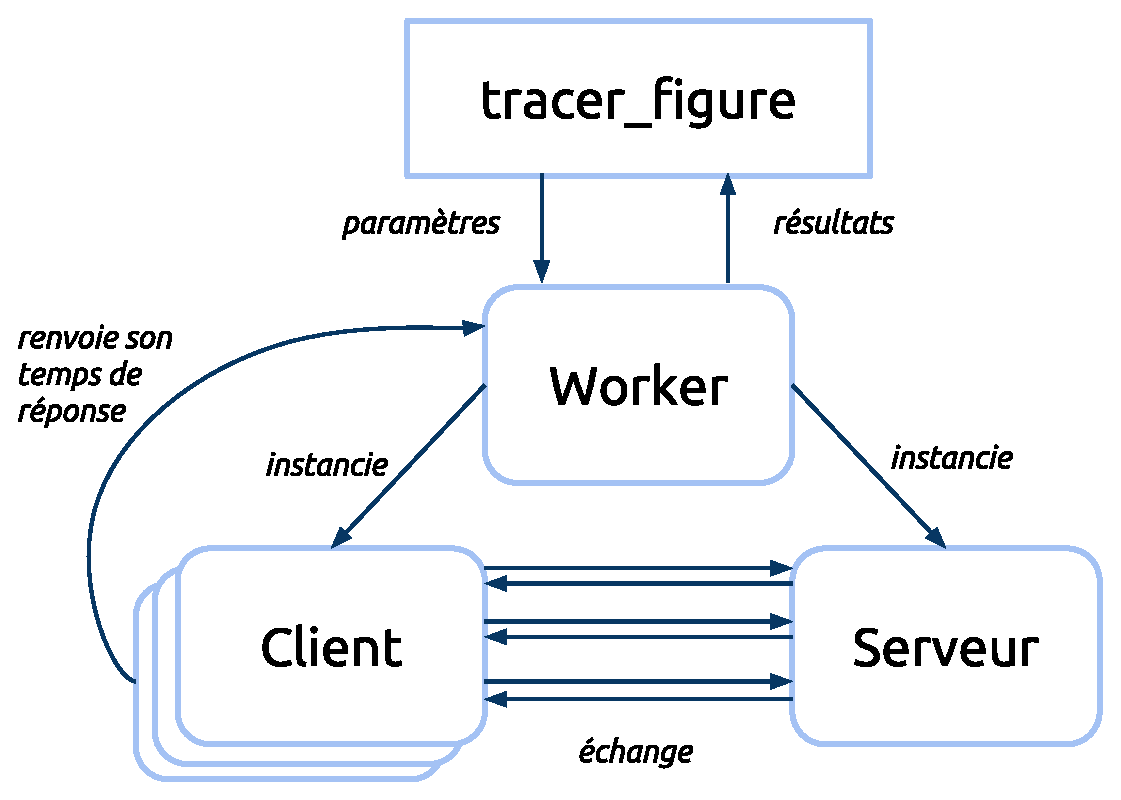
\includegraphics[scale=0.7]{image/architecture}
  \caption{Architecture du simulateur}
  \label{architecture}
\end{center}
\end{figure}

Le simulateur est programmé en \textbf{Ruby}. Il est composé de trois objets et d'un script. Le script \textit{tracer\_figure} est lancé pour effectuer les calculs et tracer les courbes, il est exécuté et s'appuie sur les objets Ruby pour calculer les temps de réponses. Le script instancie un objet \textit{Worker} qui va se charger de gérer les clients et le serveur. Le \textit{Worker} nécessite des paramètres en entrée: Le nombre de clients et le paramètre $\lambda$ du processus de Poisson pour définir la fréquence de connexion des clients. Le \textit{Worker} va ensuite instancier le \textit{Serveur} qui recevra les requêtes des \textit{Clients} et leur renverra en réponse le temps écoulé par son calcul. Le \textit{Worker} va aussi instancier plusieurs \textit{Clients} en fonction du nombre d'échantillon voulu et les connecter au \textit{Serveur} à des temps dépendant du processus de Poisson. Une fois les échanges entre \textit{Clients} et \textit{Serveur} terminés, chaque \textit{Client} va renvoyé son temps de réponse. Le \textit{Worker} renvoie ensuite ses résultats au script \textit{tracer\_figure} qui crée les courbes et analyses les statistiques.



\section{Analyse des résultats}

\end{document}
